The now well-accepted picture of neutrino mixing involves three underlying mass states, with three mixing angles defining the linear superpositions that make up each of the three weak, or flavor states.  The magnitude of the mass-squared splitting between states $\nu_1$ and $\nu_2$ is known from the KamLAND reactor experiment, and the much-larger splitting between  the third, $\nu_3$ state and the $\nu_1-\nu_2$ pair is known from atmospheric and long-baseline experiments.  However, pure neutrino oscillations are sensitive only to the magnitude of the mass splitting, not the sign.  
Defining the $\nu_1$ state as having the largest admixture of the electron flavor eigenstate, the sign of the mass splitting between states $\nu_2$ and $\nu_1$ is determined to be positive ($\Delta m^2_{21} > 0$) using the pattern of neutrino oscillations through the varying-density solar medium.
%Although it is known from the observed interactions of neutrinos with matter in the Sun that the second mass state, $\nu_2$, is heavier than the first ($\Delta m^2_{21} > 0$),  
However, the corresponding sign of $\Delta m^2_{32}\approx \Delta m^2_{31}$ remains unknown.  That is, there are two potential orderings, or ``hierarchies'', for the neutrino mass states: the so-called ``normal hierarchy'', in which $\nu_3$ is the heaviest, and the ``inverted hierarchy'', in which $\nu_3$ is the lightest (as shown in Fig.~\ref{f:hierfig}).


\begin{figure}[!ht]
\begin{center}
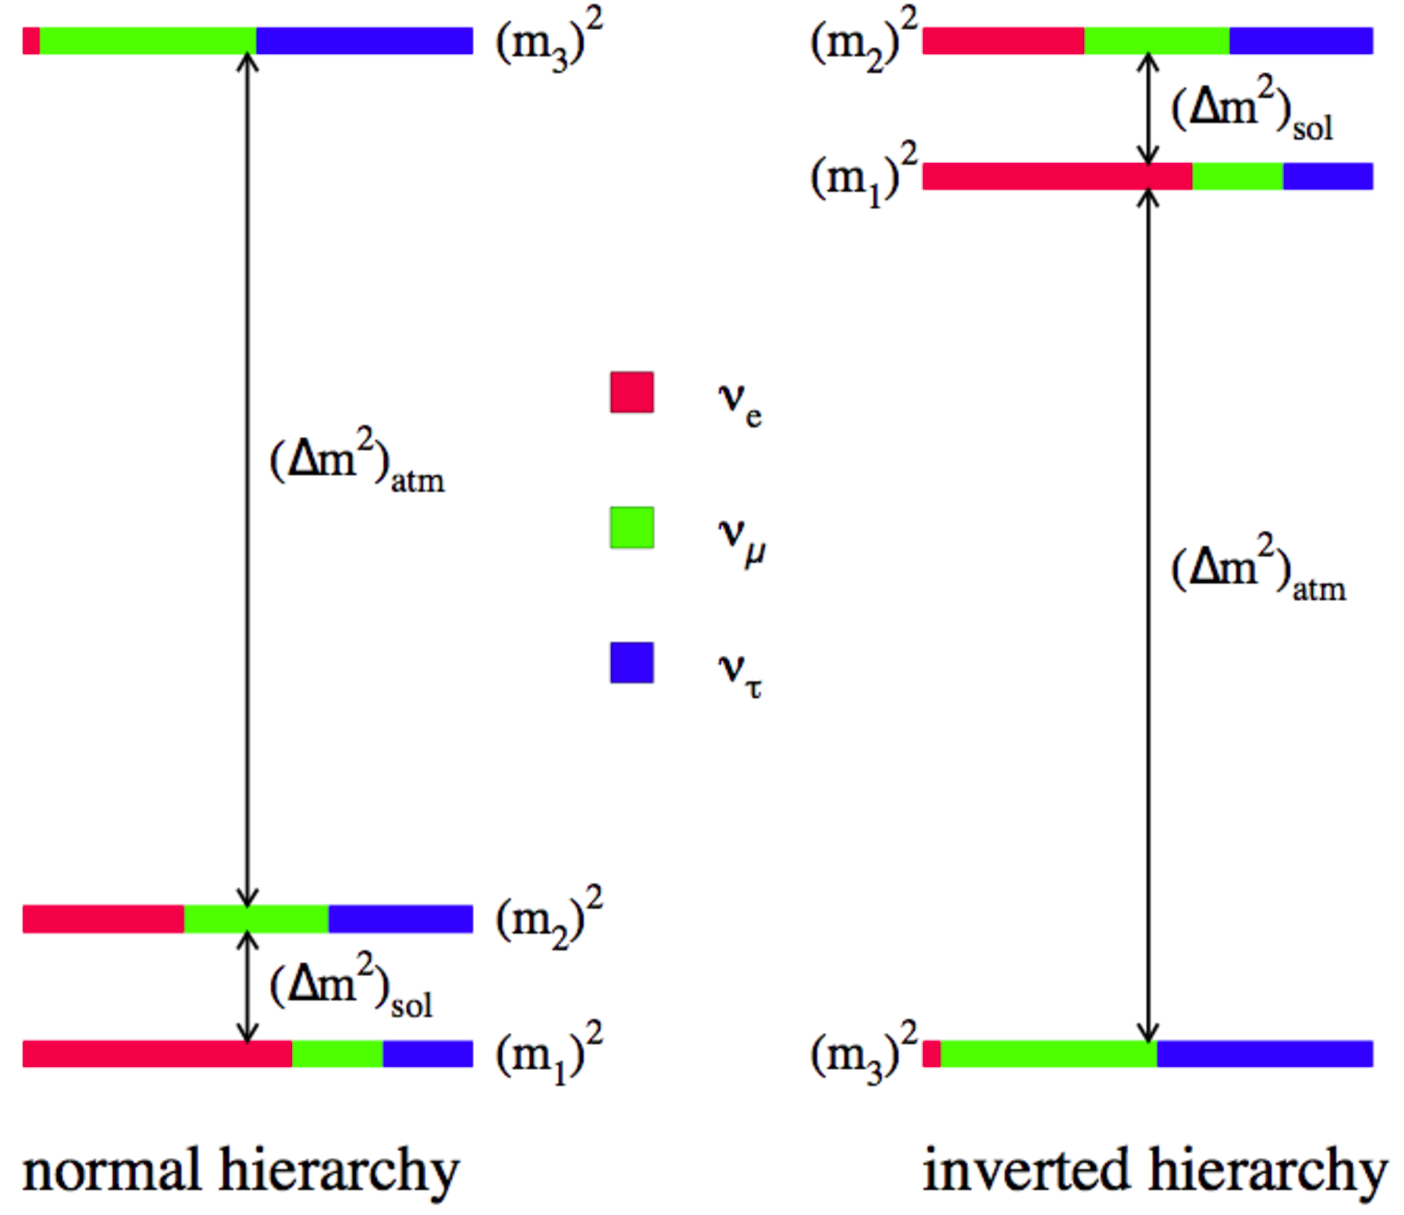
\includegraphics[width=0.55\textwidth]{./hierfig.pdf}
\caption{ Pictorial representation of the possible neutrino mass hierarchies.  Note: $\Delta m^2_{atm}$ is equivalent to $\Delta m^2_{32}$ and  $\Delta m^2_{sol}$ is equivalent to $\Delta m^2_{21}$.~\cite{gouvea}.
\label{f:hierfig}}
\end{center}
\vspace{-0.2cm}
\end{figure} 

\subsection{Status of Neutrino Mixing}\label{s:mix}

The relationship between neutrino flavor \{$\nu_e,\nu_\mu,\nu_\tau$ \} and mass \{ $\nu_1,\nu_2,\nu_3$ \} eigenstates is described 
by the PMNS mass matrix~\cite{Pontecorvo67,MNS}:
\begin{equation}
\left( \begin{array}{c} | \nu_e \rangle \\ | \nu_\mu \rangle \\ | \nu_\tau \rangle \end{array} \right) =
\left( \begin{array}{ccc} c_{12} c_{13} & s_{12} c_{13} & s_{13} e^{-i \delta_{CP}} \\
-s_{12}c_{23}-c_{12}s_{23} s_{13} e^{i \delta_{CP}} & c_{12}c_{23}-s_{12}s_{23}s_{13} e^{i \delta_{CP}} & s_{23} c_{13} \\
s_{12}s_{23}-c_{12}c_{23}s_{13} e^{i \delta_{CP}} & -c_{12}s_{23}-s_{12}c_{23}s_{13}e^{i \delta_{CP}} & c_{23} c_{13} \end{array}
\right) \left( \begin{array}{c} e^{i \alpha_1 /2} | \nu_1\rangle \\ e^{i \alpha_2 /2} | \nu_2 \rangle \\ | \nu_3 \rangle \end{array} \right)
\end{equation}
where $c_{ij} \equiv \cos{\theta_{ij}}$ and $s_{ij} \equiv \sin{\theta_{ij}}$.  
This matrix depends on:
three mixing angles $\theta_{12}$, $\theta_{13}$, and $\theta_{23}$, of which the first and last are the
dominant angles for solar and atmospheric oscillations, respectively; a Dirac phase $\delta_{CP}$ that
can induce CP-violating differences in the oscillation probabilities for
conjugate channels such as $\nu_\mu \rightarrow \nu_e$ versus
$\bar{\nu}_\mu \rightarrow \bar{\nu}_e$; and two Majorana phases $\alpha_1$ and $\alpha_2$
that will affect the interference among mass eigenstates in the effective neutrino mass probed
in the lepton-number-violating process of neutrinoless double $\beta$ decay.
%The results from solar neutrino experiments have been combined with those from reactor
%and accelerator neutrino experiments in analyses that seek (ultimately) to constrain properties of the 
%3$\times$3 neutrino mass matrix.  

%The state $\nu_1$ is the largest piece of the electron-neutrino and $\Delta m^2_{21}>0$.  One of these is by definition, while the other is an experimental fact from the observation of the MSW effect (the interaction of  neutrinos with matter) in solar neutrinos. Thus we know the sign of $\Delta m^2_{21}$, while the sign of $\Delta m_{31}^2$ is precisely the question of the neutrino mass hierarchy.  In the normal hierarchy $\Delta m_{31}^2>0$.  The  $\Delta m^2_{21}$ splitting is commonly referred to as the solar splitting, while $|\Delta m^2_{32}|$ is called atmospheric, in reference to the ways they were first observed. 


The current best knowledge of the oscillation parameters is given in Table~\ref{tab:PDGparameters}.

\begin{table}[h]\begin{center}
\caption{Neutrino parameters from~\cite{pdg}.\label{tab:PDGparameters}}
\begin{tabular}{lr}\\ \hline \hline
Parameter & Best-fit value\\ \hline
$\sin^22\theta_{12}$&$0.857 \pm0.024 $\\
$\sin^22\theta_{23}$&$>0.95$\\
$\sin^22\theta_{13}$&$ 	0.098 \pm0.013 $\\ 
$\Delta m^2_{21}$&$7.50\pm 0.20\times 10^{-5}\,{\rm eV}^2$\\
$|\Delta m^2_{32}|$&$2.32^{+0.12}_{-0.08}\times 10^{-3}\,{\rm eV}^2$\\ \hline \hline
\end{tabular}
\end{center}
\end{table}


Using these values, we find that the first maximum of oscillation, which occurs
when
\begeq
\Delta=1.27\frac{\Delta M^2({\rm eV}^2) L({\rm km})}{E({\rm GeV})}=\frac\pi{2}
\endeq 
determines the oscillation distance according to
\begeqar
L({\rm km})&=&16\times 10^3 E({\rm GeV})\\ 
                  &=&16\  E({\rm MeV})
\endeqar in the ``solar'' case while
 \begeqar
L({\rm km})&=&540\ E({\rm GeV})
\endeqar
in the ``atmospheric'' case.  With reactor neutrinos, whose typical energy is 4 MeV, the preferred distance is about 65 km for ``solar'' oscillations, while for an accelerator experiment with a typical energy of 3 GeV, we would want a distance of about 1500 km for ``atmospheric'' oscillations, or those needed to determine the sign of the $\Delta m_{31}^2$ mass splitting.

%Neutrino oscillations in vacuum are sensitive only to the magnitude of the mass splitting.  Additional oscillation caused by the interaction of neutrinos with matter provides sensitivity to the sign of the mass difference.
%To date, the only observed matter effect is in the solar neutrino sector, in which the neutrinos interact with matter as they propagate out from the Sun's core. %oscillations.  
%This is the effect that tells us the sign of $\Delta m^2_{21}$.
%Further studies in this sector provide a unique opportunity to probe the interaction of neutrinos with matter at high precision.  This is discussed in greater detail in Section~\ref{s:sol}.  The sign of the remaining mass difference, $\Delta m^2_{32}$, can be determined by terrestrial observations of the matter effect.



\subsection{Motivation for Determining the Neutrino Mass Hierarchy}\label{s:mot}
Progress in neutrino physics has been impressive over recent decades,
with the discovery of atmospheric neutrino disappearance by the
Super-Kamiokande experiment, observation of solar neutrino flavor
change by the Sudbury Neutrino Observatory (SNO), and final
confirmation of the phenomenon of neutrino oscillation by the KamLAND
reactor neutrino experiment, which observed both disappearance and
reappearance.  More recently, the final mixing angle, $\theta_{13}$, 
has been determined by the Daya Bay collaboration to be large:
$\sin^22\theta_{13}=0.089\pm0.010\,\textrm{(stat)}\,\pm0.005\,\rm(syst)$~\cite{DB},
an observation subsequently confirmed by RENO~\cite{Reno} and others. 

%LBNL played a leading role in three of these four ground-breaking experiments, and is thus well positioned to lead efforts to determine the mass hierarchy.

%Despite these leaps forward in understanding, several fundamental questions remain unanswered:  what is the absolute neutrino mass scale?  Do neutrinos violate CP?  Are neutrinos Dirac or Majorana?  Greater precision in neutrino-oscillation parameter measurements would allow tests of symmetries with quark mixing, and sensitive searches for new physics.  And, finally, the unique nature of neutrinos allows them to be used to probe otherwise unreachable parts of the universe: from the Earth beneath our feet to the center of the Sun and far-distant supernovae.
%Knowledge of the neutrino mass hierarchy  can help to inform each of these questions.
Once we understand the ordering of the neutrino mass states, the uncertainty on a measurement of the  CP-violating phase, $\delta_{CP}$, is significantly reduced.   
Knowledge of the mass hierarchy would define the scope for future neutrinoless double beta decay ($0\nu\beta\beta$) experiments, seeking to resolve the mass nature of the neutrino, by limiting the domain for observation of a signal.  In combination with cosmological measurements, which are sensitive to the sum of neutrino masses, knowledge of the mass hierarchy could also be used to determine the absolute mass scale of neutrinos.
The mass hierarchy could also further understanding of core-collapse supernovae.  
For these many reasons, determination of the neutrino mass hierarchy is thus a fundamental step towards completion of the Standard Model of particle physics.  



